\documentclass[10pt,twocolumn]{article}
\usepackage{graphicx}
\usepackage{amsmath}
\usepackage{booktabs}
\usepackage[margin=0.5in, top=0.2in, bottom=0.5in]{geometry}
\usepackage{authblk}
\usepackage{hyperref}
\usepackage{float}
\usepackage{caption}
\usepackage{subcaption}
\usepackage{cleveref}

% Handle figures in two-column layout better
\usepackage{stfloats}

% Title formatting
\title{\Large \textbf{Neuron Responses to Grating Stimulus Orientations in Mice}}

\author{
  Umut Tuna Akgul, Utku Bahcivanoglu, Tommaso Ferracina, George Morris, Tebe Nigrelli
}


\begin{document}

\maketitle

\begin{abstract}
We analyze ecephys data from the Allen Brain Observatory to investigate how neural units in the mouse visual cortex respond to static and drifting gratings stimuli. We identify brain regions and specific neurons that have a significant role in encoding stimulus orientation. We combine neural firing rate over multiple trials and conditions, and select the most informative neurons based on their response. Finally, we construct an  effective decoder to predict stimulus orientation from neural activity.
\end{abstract}


\section{Data Processing}

We selected session \textit{750332458} from the \textit{AllenSDK} dataset for its balanced presence of units between regions, especially those related to the visual cortex \ref{tab:regions}. The dataset consists of time-aligned responses of neuronal units to stimuli. We restrict the data to firing rate as the only feature, grouping responses by stimulus orientation, and focusing our study on the mean firing rate of each unit - neuron.

\section{Exploratory Data Analysis}

We observe how spiking rate varies between regions: in general, we notice a linear relation between the log of the mean and the log of the standard deviation of the firing rates. Visually, it is clear that simply observing mean and standard deviation is not enough to characterize the brain region \ref{fig:firing_rate_stats}, though some qualitative differences can be identified. As some regions contain little data, spread is subject to noise \ref{fig:firing_rate_single}.

\subsection{Decoding static vs drifting}

As a preliminary step, we study spike count and trial variability between static and drifting stimuli in the visual cortex - VISam. In the same unit, spike count per presentation (spike mean) is much higher in the drifting stimulus \ref{fig:spike_mean}. Testing this with a paired Wilcoxon signed-rank test reveals a p-value of 0, showing a uneven firing rates between static and drifting. We then perform the same analysis on spike Coefficient of Variation, showing the opposite: units have greater variability when presented with static gratings (p-value 0) \ref{fig:spike_cv}.

For reference, we trained a Random Forest classifier with 5-fold training to predict static from drifting, given either spike\_mean or spike\_CV: spike\_mean gave an accuracy of 1 and spike\_CV attained 0.93.

\section{Selection of Neurons}

We use the Orientation Selectivity Index (OSI) to identify a highly selective subset of neurons (OSI $>$ 0.5).

We used one-way ANOVA test for validation, comparing spike counts across different orientations, taking as null hypothesis that mean is equal across all orientations. The test identified a substantial population of neurons (p $<$ 0.05) exhibiting statistically significant orientation tuning.

We selected neurons with High orientation selectivity and Statistically significant orientation tuning.

\subsection{Static}

This approach yielded a population of 43 orientation-selective neurons distributed in the visual cortex, with notable concentrations in the VISal and VISl areas. The anatomical distribution of these neurons aligns with established literature on the hierarchical organization of orientation processing in the mouse brain.

Visualization of orientation tuning curves from representative neurons revealed diverse response profiles, including: narrowly tuned neurons with a strong response to one specific orientation, and Neurons with a broader reaction to a few concurrent orientations.

These different tuning properties are likely beneficial to the encoding of orientation in the visual cortex, helping to discriminate between different orientations of visual stimuli. Tuning curves for static gratings can be found in Figure \ref{fig:static_tuning} in Appendix A.

\subsection{Drifting}

The same approach for drifting gratings was then employed with the same selection criteria. It revealed 81 orientation-selective neurons (almost double) many of which had higher OSI values between 0.8-1.0. Similarly, all were located in the visual cortex, predominantly in VISal, bar one which was in 'grey'.

The tuning curves were similarly conveying diverse response profiles with very strong responses to specific orientations \ref{fig:drifting_tuning}. Though, the drifting tuning curves showed more peakedness around the preferred orientation, this is probably largely due to the fact that the difference between adjacent orientations is 45° instead of 30° and is not solely because the grating is drifting.

\begin{figure}[h]
  \centering
  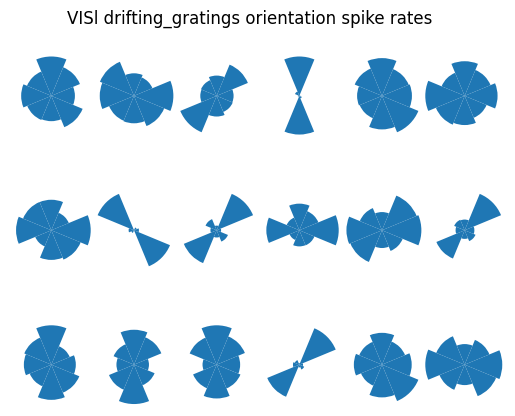
\includegraphics[width=0.6\linewidth]{report_images/drifting_unit_mean_orientation.png}
  \caption{Mean orientation preference of drifting units}
  \label{fig:drifting_unit_mean_orientation}
\end{figure}

Moreover, unlike Static here the orientations spanned a full 360° with the 45° increments giving 8 different orientations. A very interesting result was that orientations 180° apart both had very strong responses, where the gratings has the same orientation but is drifting in the opposite direction \ref{fig:drifting_unit_mean_orientation}. Indeed it seems the units in general seemed to be more selective to orientation than direction. We wanted to test this by investigating DSI (Direction-sensitivity index).

Using the same selection criteria above except using DSI $>$ 0.5 instead only 8 neurons were left over supporting this hypothesis.

\section{Decoding Orientation from Neural Activity}

To assess whether the activity patterns of orientation-selective neurons could reliably predict stimulus orientation, we implemented a machine learning approach using the spike counts of selected neurons as features. The static dataset consisted of spike count responses to static grating stimuli presented at six distinct orientations. Whereas the drifting dataset the same but from 8 distinct orientations as direction is considered. The classification task involved predicting the stimulus orientation from the corresponding neural activity patterns.

\subsection{Data Preparation and Model Training}
We constructed a feature matrix with stimulus presentations as rows and the spike counts of a selected neurons as columns with the orientation values being the target variable. Prior to model training the dataset was stratified and split into training (70\%) and testing (30\%) sets to ensure proportional representation of orientation classes. We ended up with 20 presentations per orientation for static dataset whereas only 5 presentations per orientation for drifting dataset, a limitation to be considered. Features were standardized using z score normalization to account for differences in baseline firing rates. We then considered Random Forest Models, SVM with linear kernel and Logistic Regression.

\subsection{Classification performance}

For static, all models performed with accuracy near 0.85 \ref{tab:static_performance}, while drifting performed with near perfect accuracy \ref{tab:drifting_performance}. In both datasets, logistic regression performed best. The difference in performance can be explained by having more orientation-selective features (81 from 43), with these neurons having higher OSI values, though it must be acknowledged that the resolution changes between grating types, possibly affecting decoding. Moreover, our model is limited by having 5 stimulus presentations for drifting and 20 for static.

\subsection{Cross condition analysis between static and drifting stimuli}

At this point we wanted to dig deeper into the difference in OSI between static and drifting gratings by looking at the distribution of the OSI values \ref{fig:tuning_comparison}. 

\[
\begin{array}{|l|c|c|}
\hline
\textbf{Measure} & \textbf{Static Gratings} & \textbf{Drifting Gratings} \\
\hline
\text{Skewness} & 2.258 & 1.937 \\
\text{Kurtosis} & 5.009 & 3.397 \\
\hline
\end{array}
\]

The distribution is highly non-normal: few neurons have a high OSI and are responsible for interpreting orientation.

Drifting activates more neurons with high OSI overall.

Static distribution has higher kurtosis (5.009 $>$ 3.397) indicating a narrower sharper peak and heavier tails than drifting. This suggests fewer relatively higher tuned neurons: the drifting nature of the grating is a kind of noise which triggers a greater response.

Interestingly we see these results in the feature selection of our random forest models for static and drifting. For static fewer units make up a relatively much larger impact on the models decision than for drifting gratings. As for drifting many units have a high OSI value. 

\subsubsection{Distribution and Overlap of Selective Neurons Across Regions}

The distribution of well-tuned neurons across brain regions is very similar, with approximately twice as many well-tuned neurons for drifting compared to static gratings \ref{fig:tuned_regions}. Notably, VISl appears to have greater relative importance for static stimuli, whereas VISrl is more prominent for drifting. Furthermore, of the 43 units identified as significant for static gratings, 29 were also significant for drifting gratings. This substantial overlap indicates that many of the same neurons are involved in processing orientation for both stimulus types, which aligns with expectations.

\section{Limitations and Further Work}

Comparing model performance between static and drifting gratings is limited by the high discrepancy in resolution: static has 30° and while 45° in drifting. This does not limit comparative analysis for OSI as this uses orthogonal values for stimulus count, the same for both. A comparative study with the same resolution could refine our results.

This investigation was limited to a single session, for a mouse. Repeating the study with other sessions would validate results.

We used gratings to infer how orientation is encoded, but it remains to be validated if other oriented stimuli are similarly encoded.

\section{Conclusion}

It is possible to decode gratings orientation from neural response using spike counts. This method is especially effective in drifting gratings, where units have higher OSI values and are selective. However, OSI values for selective neurons in static gratings are much higher, as is apparent from higher kurtosis, and is confirmed by feature importance in the model.

\newpage

\appendix

\section{Appendix}

\begin{table}[H]
\centering
\begin{tabular}{lr}
\toprule
region & count \\
\midrule
grey   & 558 \\
VISal  &  71 \\
VISp   &  63 \\
VISam  &  60 \\
VISrl  &  44 \\
VISl   &  38 \\
VISpm  &  19 \\
CA1    &  16 \\
CA3    &  15 \\
DG     &   7 \\
\bottomrule
\end{tabular}
\caption{Distribution of units across brain regions.}
\label{tab:regions}
\end{table}

\begin{figure}[H]
\centering
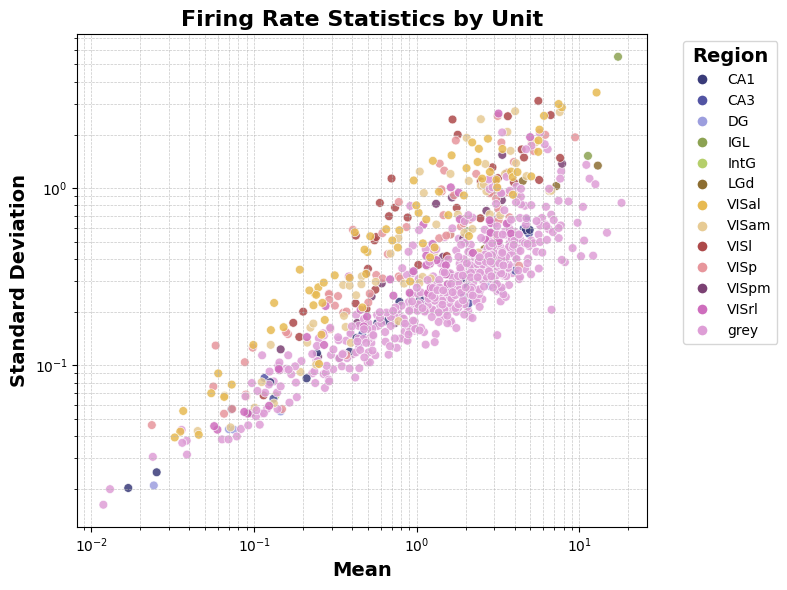
\includegraphics[width=\linewidth]{report_images/unit_firing_rate_statistics.png}
\caption{Firing rate statistics across brain regions.}
\label{fig:firing_rate_stats}
\end{figure}

\begin{figure}[H]
\centering
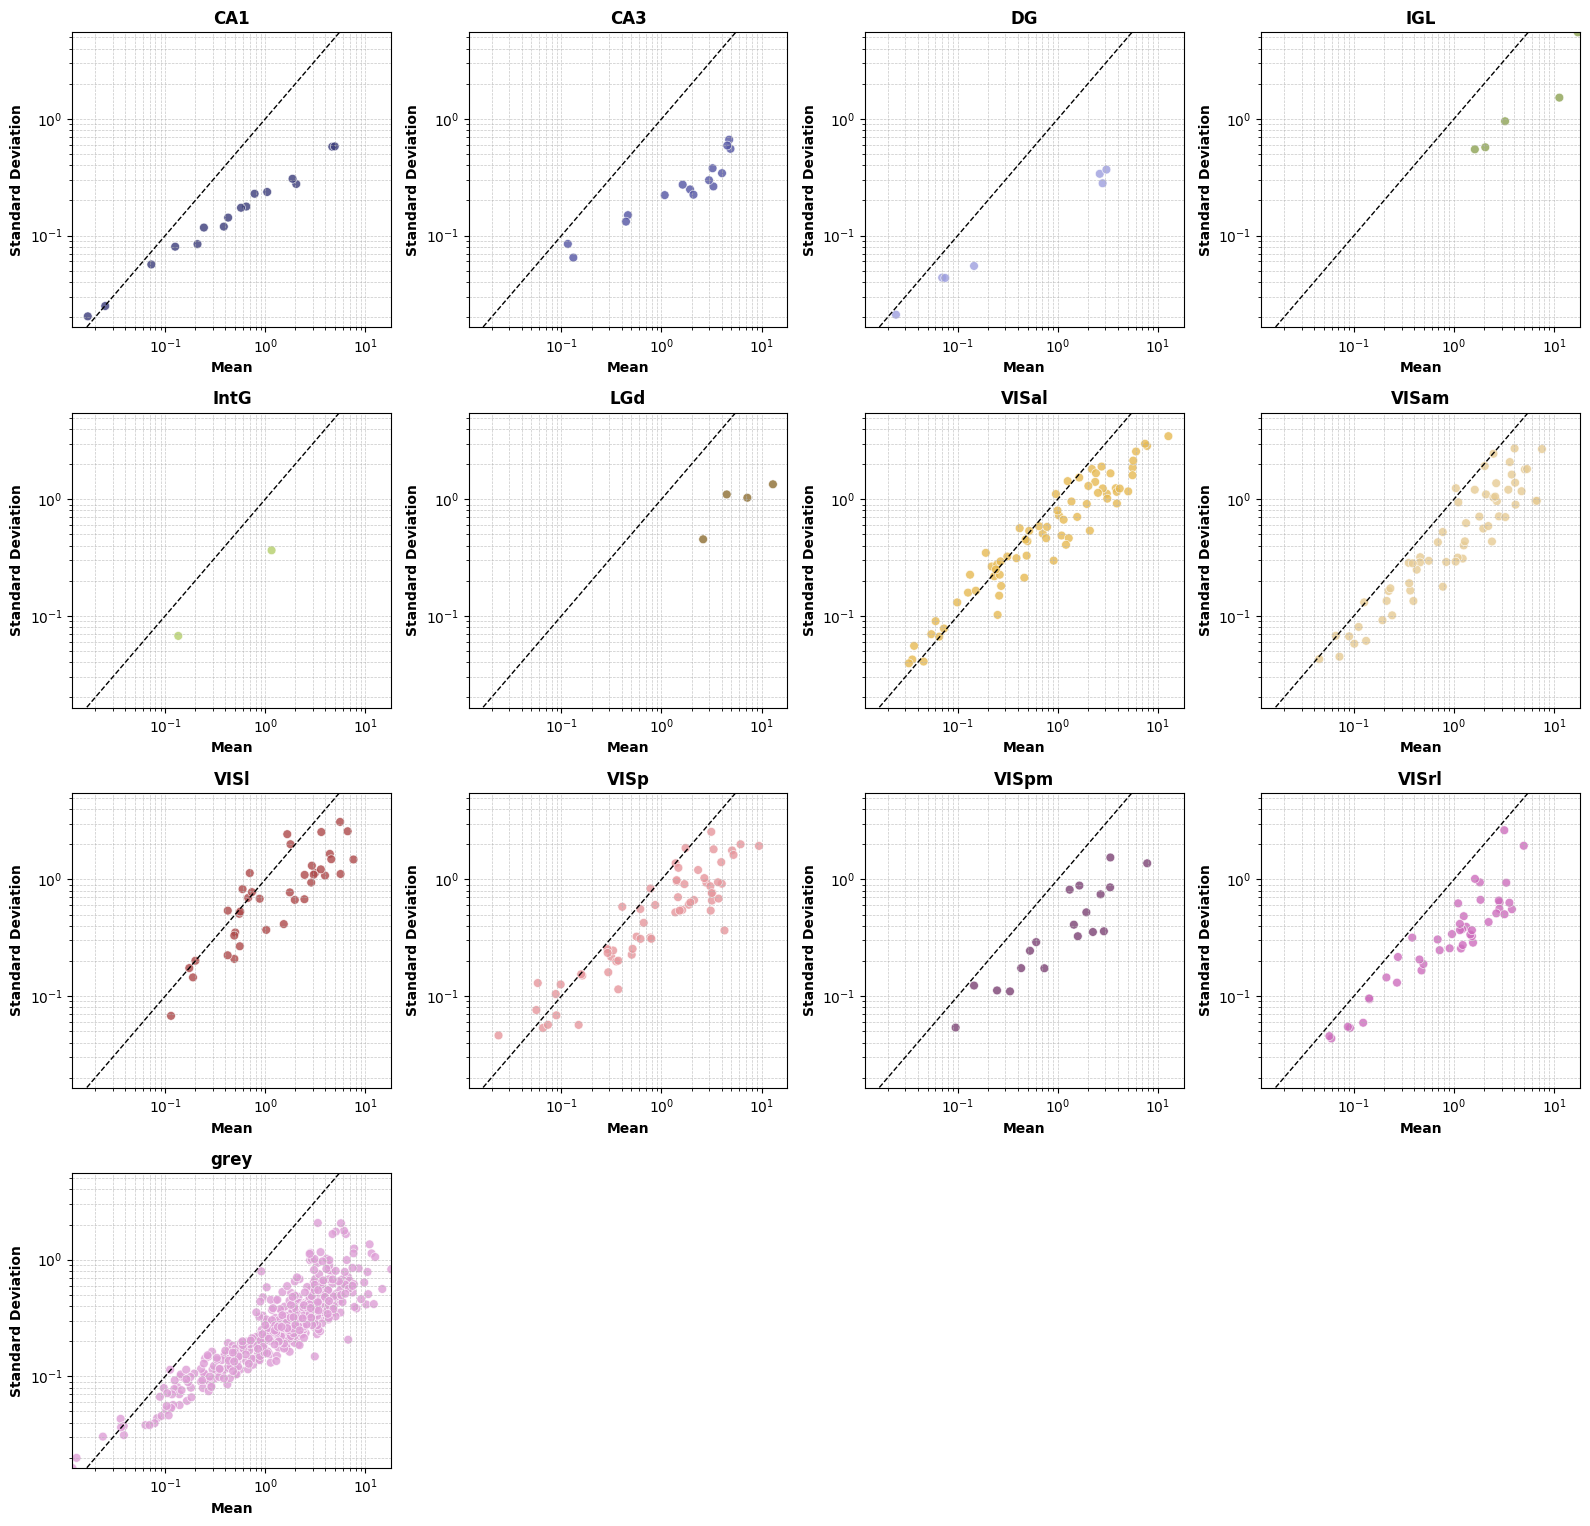
\includegraphics[width=\linewidth]{report_images/unit_firing_rate_statistics_single.png}
\caption{Individual firing rate statistics for each brain region.}
\label{fig:firing_rate_single}
\end{figure}

\begin{figure}[H]
  \centering
  \begin{subfigure}[b]{0.48\linewidth}
    \centering
    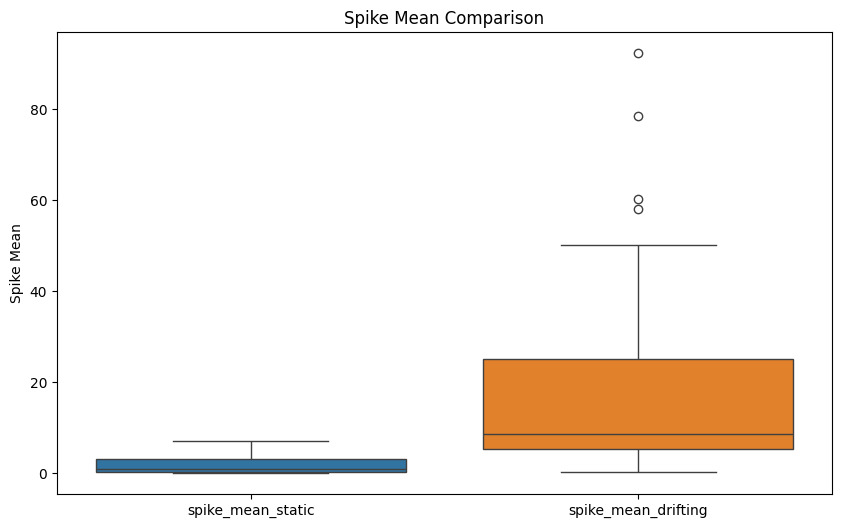
\includegraphics[width=\linewidth]{report_images/spike_mean_comparison.png}
    \caption{Spike mean: static, drifting}
    \label{fig:spike_mean}
  \end{subfigure}
  \hfill
  \begin{subfigure}[b]{0.48\linewidth}
    \centering
    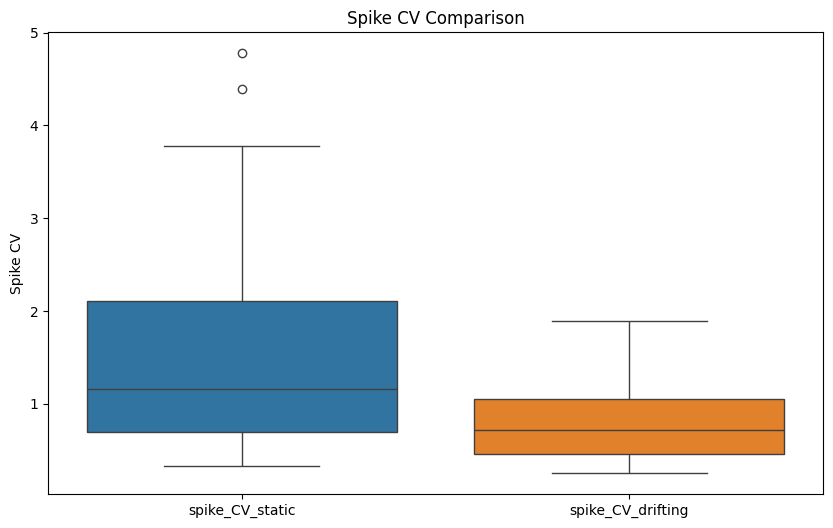
\includegraphics[width=\linewidth]{report_images/spike_CV_comparison.png}
    \caption{Spike CV: static and drifting}
    \label{fig:spike_cv}
  \end{subfigure}
  \caption{Comparison of spike mean and coefficient of variation between static and drifting gratings.}
  \label{fig:spike_stats_comparison}
\end{figure}


\begin{figure}[H]
\centering
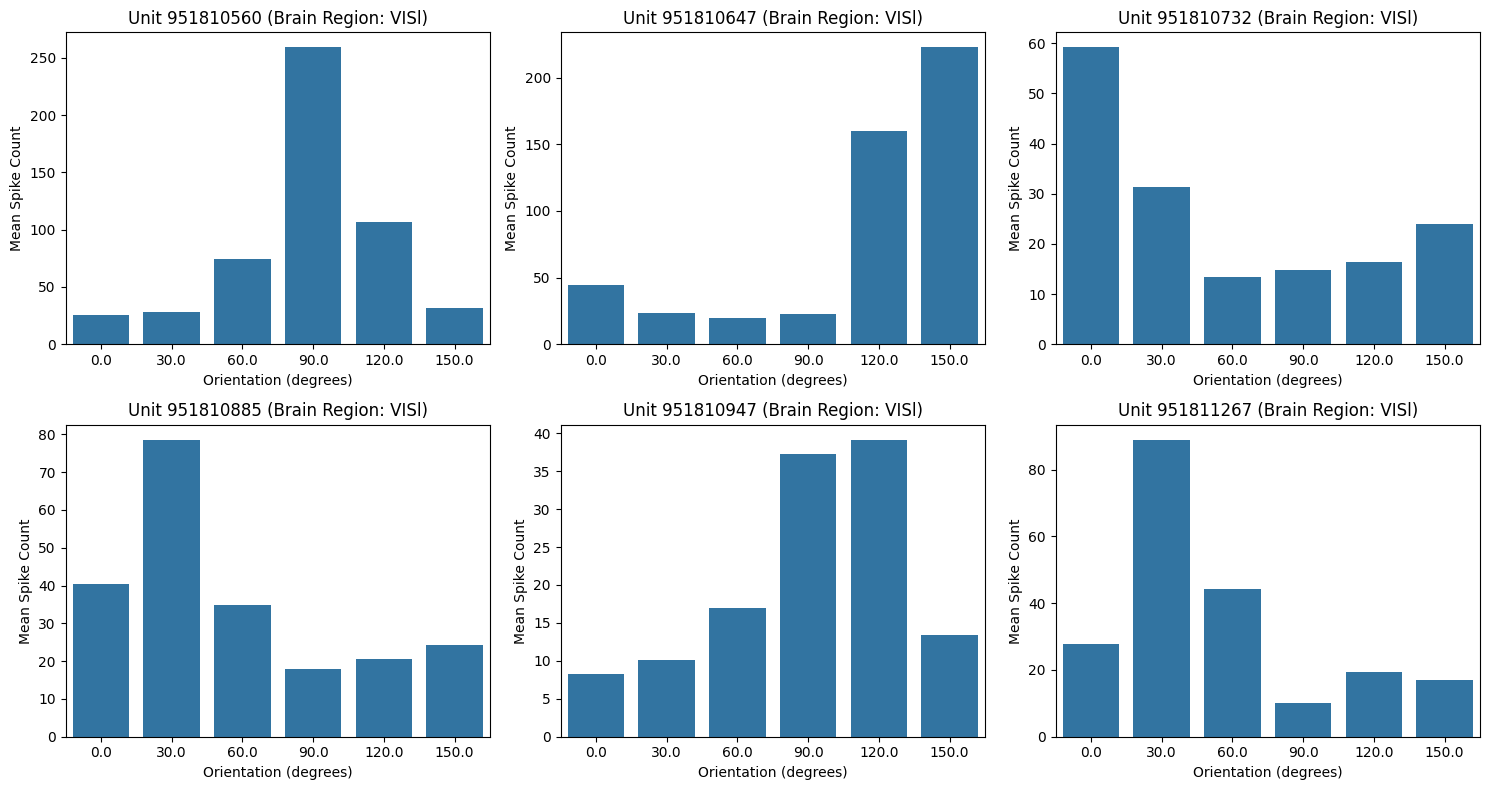
\includegraphics[width=\linewidth]{report_images/static_tuning_curves.png}
\caption{Tuning curves for static gratings.}
\label{fig:static_tuning}
\end{figure}

\begin{figure}[H]
\centering
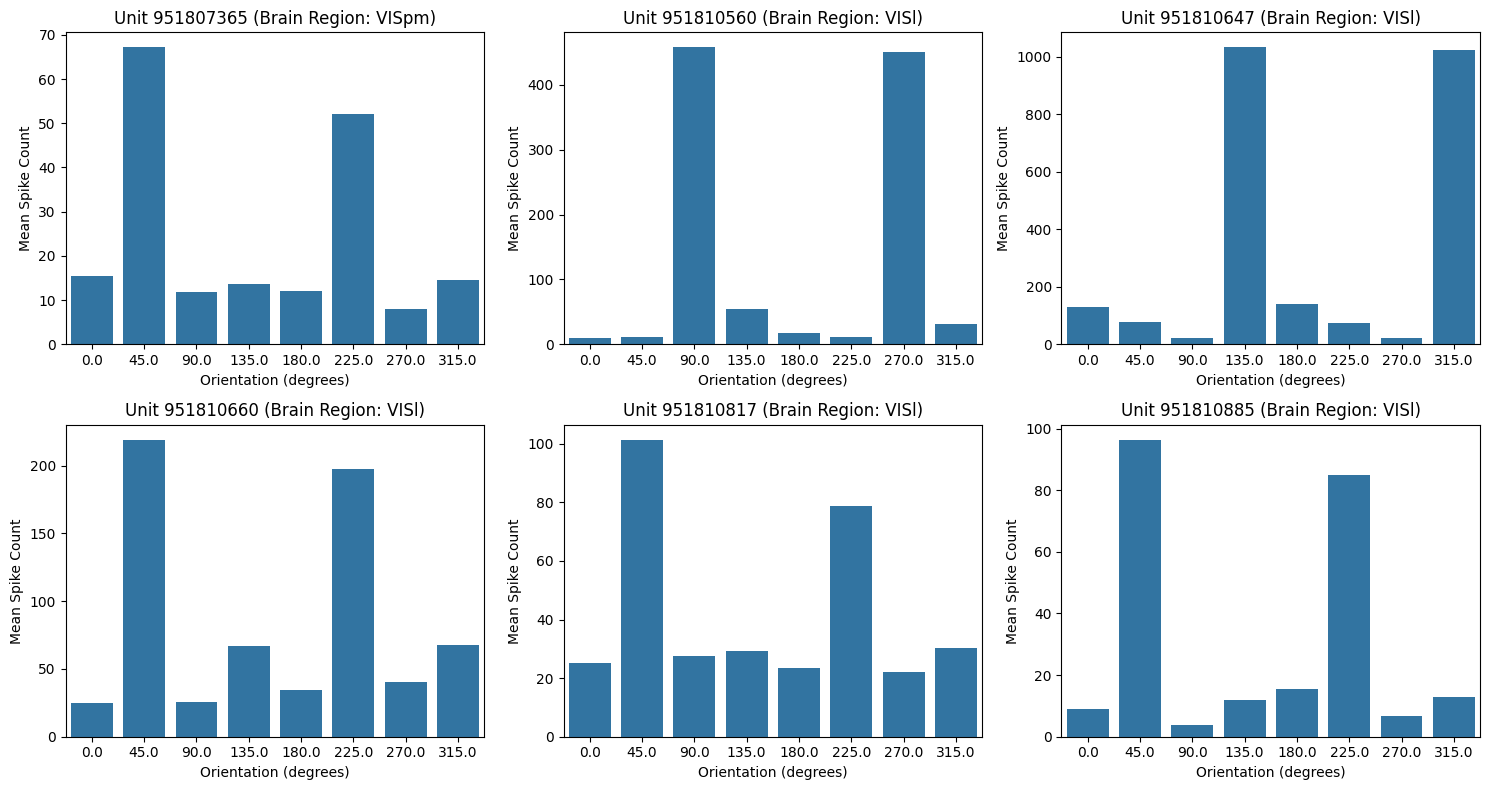
\includegraphics[width=\linewidth]{report_images/Drifting_tuning_curves.png}
\caption{Tuning curves for drifting gratings.}
\label{fig:drifting_tuning}
\end{figure}

\begin{figure}[H]
  \centering
  \begin{subfigure}[b]{0.48\linewidth}
    \centering
    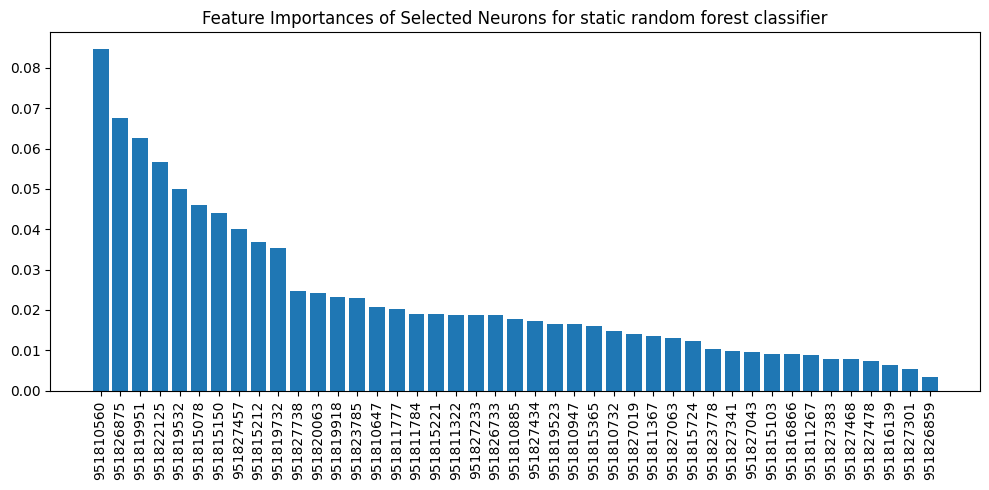
\includegraphics[width=\linewidth]{report_images/static_feature_selection.png}
    \caption{Static gratings}
    \label{fig:static_feature}
  \end{subfigure}
  \hfill
  \begin{subfigure}[b]{0.48\linewidth}
    \centering
    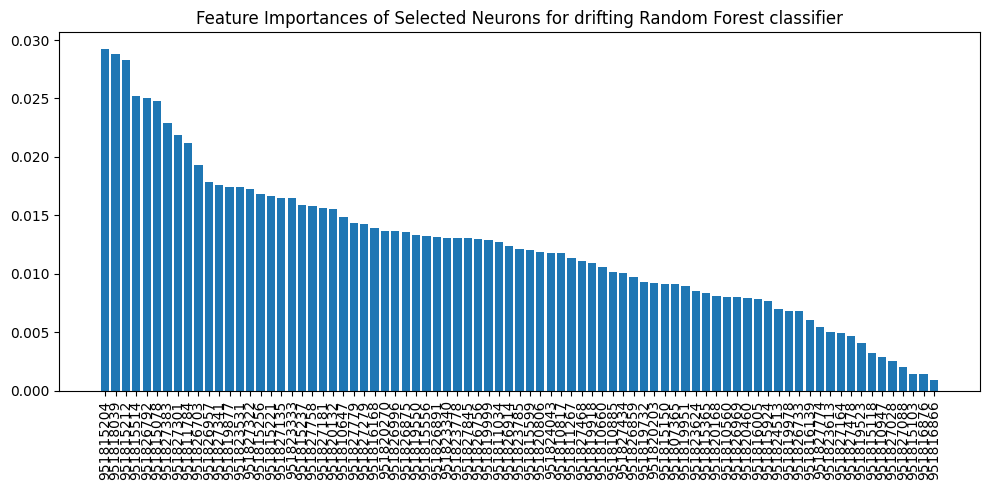
\includegraphics[width=\linewidth]{report_images/drifting_feature_selection.png}
    \caption{Drifting gratings}
    \label{fig:drifting_feature}
  \end{subfigure}
  \caption{Feature selection results for static and drifting gratings.}
  \label{fig:feature_selection_comparison}
\end{figure}


\begin{figure}[H]
  \centering
  \begin{subfigure}[b]{0.48\linewidth}
    \centering
    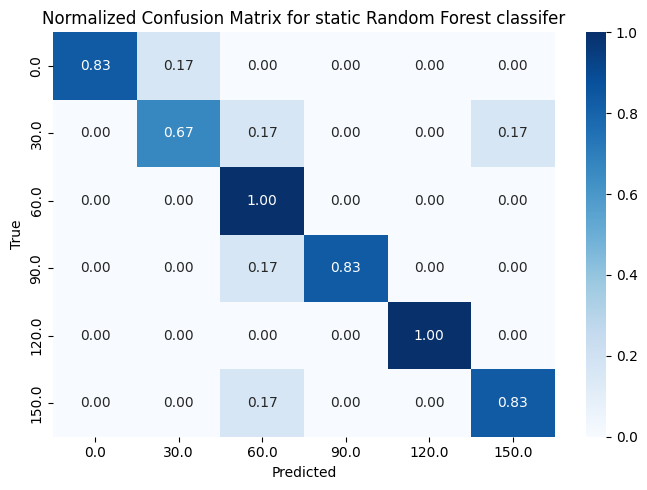
\includegraphics[width=\linewidth]{report_images/static_random_forest_confusion_matrix.png}
    \caption{Static gratings}
    \label{fig:static_rf_cm}
  \end{subfigure}
  \hfill
  \begin{subfigure}[b]{0.48\linewidth}
    \centering
    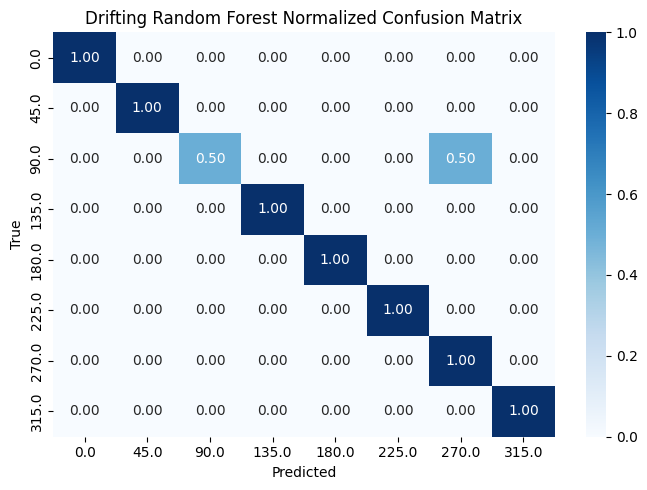
\includegraphics[width=\linewidth]{report_images/drifting_random_forest_confusion_matrix.png}
    \caption{Drifting gratings}
    \label{fig:drifting_rf_cm}
  \end{subfigure}
  \caption{Random Forest confusion matrices for static and drifting gratings.}
  \label{fig:rf_cm_comparison}
\end{figure}  

\begin{figure}[H]
\centering
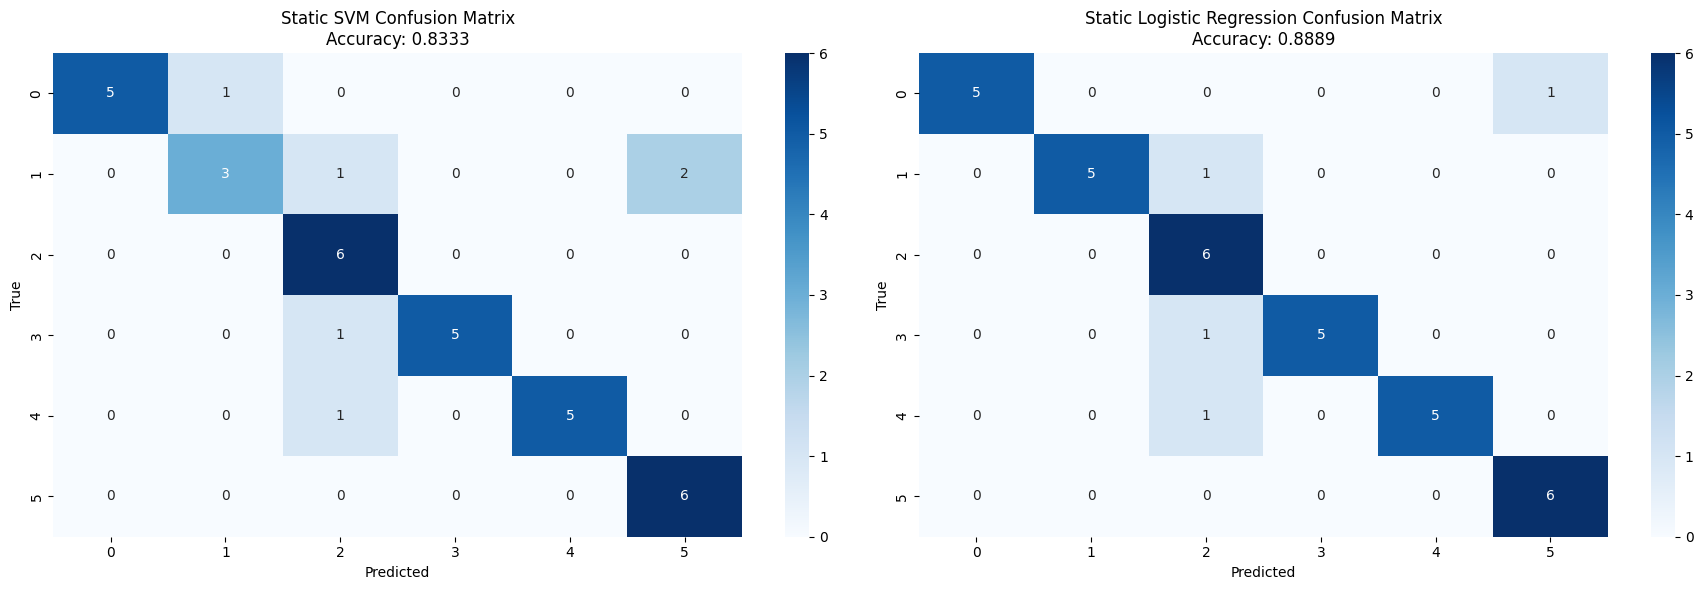
\includegraphics[width=\linewidth]{report_images/static_SVM_LogR_confusion_matrix.png}
\caption{SVM and Logistic Regression confusion matrices for static gratings.}
\label{fig:static_svm_logr_cm}
\end{figure}


\begin{table}[H]
  \centering
  \begin{tabular}{l c}
  \hline
  \textbf{Static} & \textbf{Accuracy} \\
  \hline
  Random Forest        & 0.8611 \\
  SVM                  & 0.8333 \\
  Logistic Regression  & 0.8889 \\
  \hline
  \end{tabular}
  \caption{Classification accuracy for static gratings.}
  \label{tab:static_performance}
  \end{table}
    
  Feature selection for static gratings is visualized in Figure \ref{fig:static_feature} in Appendix A. The confusion matrices for Random Forest, SVM, and Logistic Regression models for static gratings are presented in Figures \ref{fig:static_rf_cm} and \ref{fig:static_svm_logr_cm} in Appendix A.
  
  \begin{table}[H]
  \centering
  \begin{tabular}{l c}
  \hline
  \textbf{Drifting} & \textbf{Accuracy} \\
  \hline
  Random Forest        & 0.9167 \\
  SVM                  & 1.0000 \\
  Logistic Regression  & 1.0000 \\
  \hline
  \end{tabular}
  \caption{Classification accuracy for drifting gratings.}
  \label{tab:drifting_performance}
  \end{table}
  
  Feature selection for drifting gratings is visualized in Figure \ref{fig:drifting_feature} in Appendix A. The confusion matrices for Random Forest, SVM, and Logistic Regression models for drifting gratings are presented in Figures \ref{fig:drifting_rf_cm} and \ref{fig:drifting_svm_logr_cm} in Appendix A.  

\begin{figure}[H]
\centering
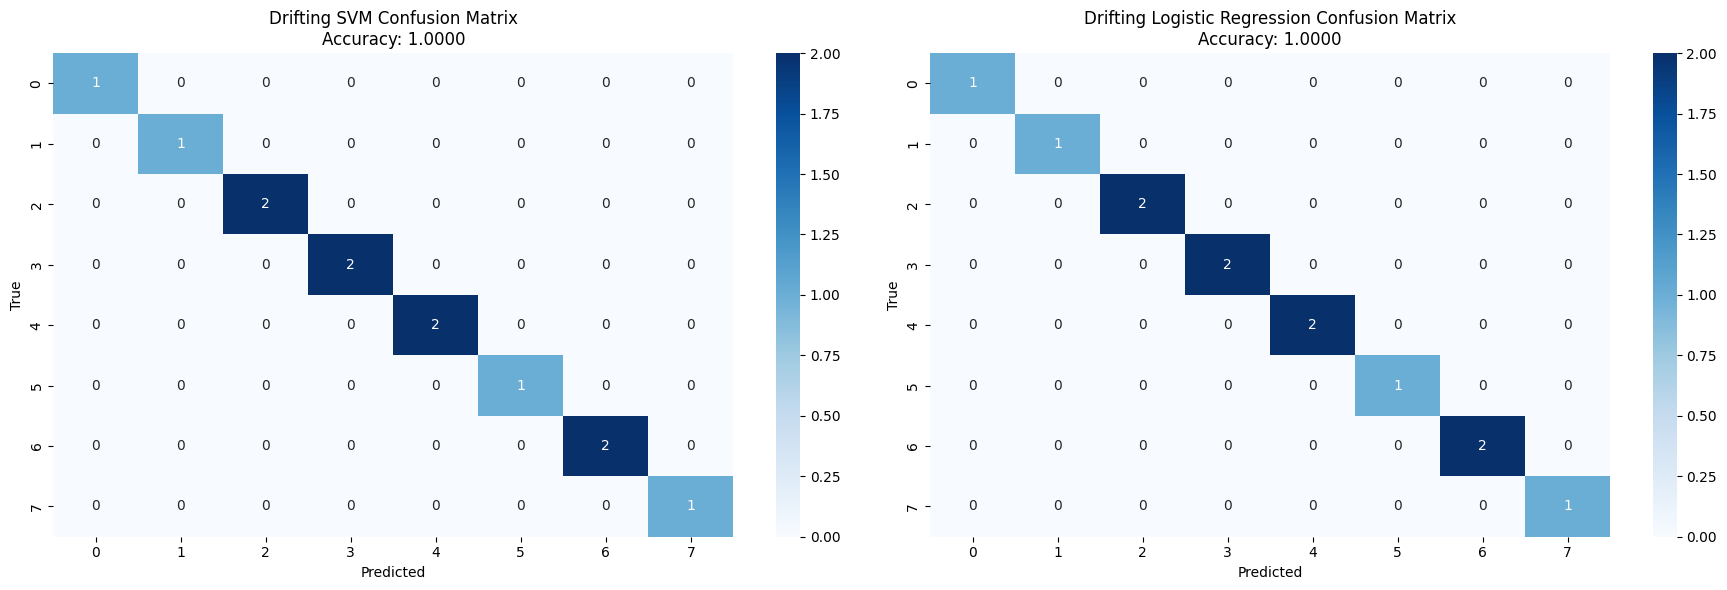
\includegraphics[width=\linewidth]{report_images/drifting_SVM_LogR_confusion_matrix.png}
\caption{SVM and Logistic Regression confusion matrices for drifting gratings.}
\label{fig:drifting_svm_logr_cm}
\end{figure}

\begin{figure}[H]
  \centering
  \begin{subfigure}[b]{0.48\linewidth}
    \centering
    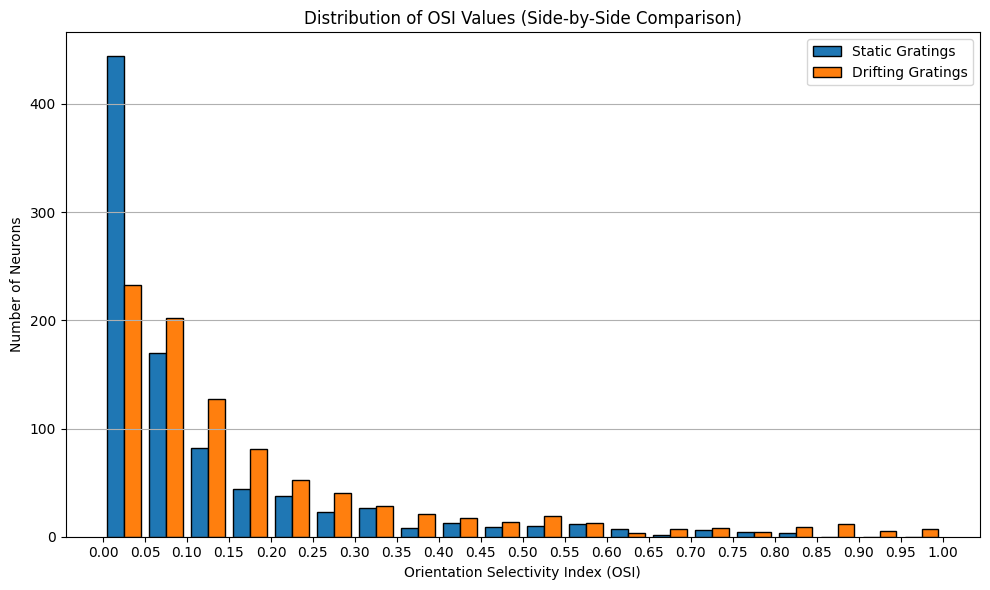
\includegraphics[width=\linewidth]{report_images/tuning_curves_comparison.png}
    \caption{Tuning curves: static vs. drifting.}
    \label{fig:tuning_comparison}
  \end{subfigure}
  \hfill
  \begin{subfigure}[b]{0.48\linewidth}
    \centering
    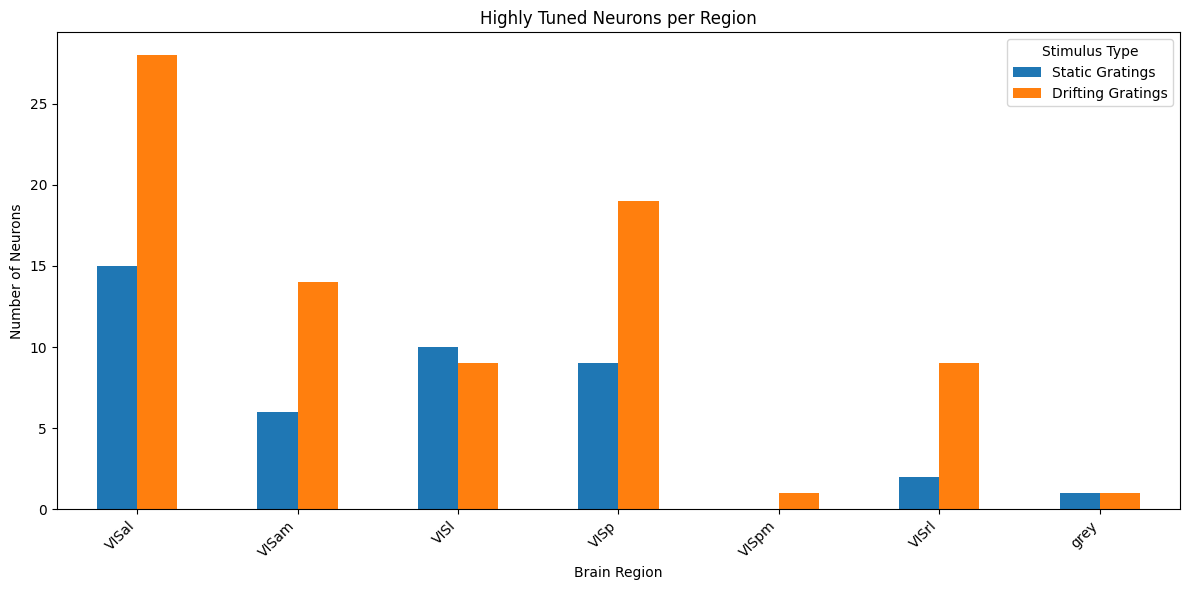
\includegraphics[width=\linewidth]{report_images/tuned_neurons_region.png}
    \caption{Orientation-selective neurons by region.}
    \label{fig:tuned_regions}
  \end{subfigure}
  \caption{Comparison of tuning responses and regional distribution of orientation-selective neurons.}
  \label{fig:tuning_summary}
\end{figure}

\end{document}